% Copyright (c) 2010 Jérémie DECOCK (http://www.jdhp.org)

% This document is provided under the terms of the "Creative Commons BY-SA" license.
% For more details, read "legalcode.html" enclosed file or "http://creativecommons.org/licenses/by-sa/2.0/fr/" web page.

\documentclass{beamer}
\usepackage[utf8]{inputenc}
\usepackage[frenchb]{babel}
\usepackage{hyperref}
\usepackage{subfigure}
%\usepackage[pdftex]{graphicx}
%\usepackage{natbib}
\usepackage{listings}
%\usepackage{algorithmic}
\usepackage{calc}

\lstset{
    basicstyle=\small,                                % print whole listing small
    keywordstyle=\color{black}\bfseries\underbar,     % underlined bold black keywords
    identifierstyle=,                                 % nothing happens
    commentstyle=\color{white},                       % white comments
    stringstyle=\ttfamily,                            % typewriter type for strings
    showstringspaces=false                            % no special string spaces
}


\hypersetup{
	pdftoolbar=true,                                          % show Acrobat’s toolbar ?
	pdfmenubar=true,                                          % show Acrobat’s menu ?
	pdffitwindow=true,                                        % page fit to window when opened
	pdftitle={La coordination d'agents dans le cadre d'un jeu de football},                                % title
	pdfauthor={Jérémie DECOCK},                                                                               % author
	pdfsubject={La coordination d'agents dans le cadre d'un jeu de football},  % subject of the document
	pdfnewwindow=true,                                                                                        % links in new window
	pdfkeywords={Système multi-agents, coordination, roboskeleton, football, robocup},                               % list of keywords
	colorlinks=true,                                          % false: boxed links; true: colored links
	linkcolor=black,                                          % color of internal links
	citecolor=black,                                          % color of links to bibliography
	filecolor=black,                                          % color of file links
	urlcolor=black                                            % color of external links
}

%\usetheme{Singapore}

\title{La coordination d'agents dans le cadre d'un jeu de football}
\author{Jérémie \bsc{Decock}}
\institute{UPMC}
\date{18 mars 2010}

\begin{document}

\begin{frame}
\titlepage
\end{frame}

%%%%%%%%%%%%%%%%%%%%%%%%%%%%%%%%%%%%%%%

\begin{frame}
\frametitle{Plan}
%\tableofcontents
\tableofcontents[sectionstyle=show/show,subsectionstyle=hide/hide/hide]
\end{frame}

%%%%%%%%%%%%%%%%%%%%%%%%%%%%%%%%%%%%%%%

\section{Introduction}
\begin{frame}
\begin{center}
{\LARGE Introduction}
\end{center}
\end{frame}


\begin{frame}
\frametitle{Introduction}
Deux championnats internationaux
\begin{itemize}
	\item Robocup (Robot Soccer World Cup) $[$KIT98$]$
	\item FIPA (Federation of International Robot-soccer Association)
\end{itemize}
~\\
Des enjeux sérieux
\begin{itemize}
	\item tester et confronter les travaux de différents laboratoires dans de nombreux domaines
    \item une tâche difficile et réaliste (transposable sur des problèmes plus concrets)
    \item plusieurs ligues pour aborder différents problèmes en parallèle (de la motricité à la coordination entre agents)
\end{itemize}
\end{frame}


\begin{frame}
\frametitle{Introduction}
\begin{figure}
    \centering
    \subfigure{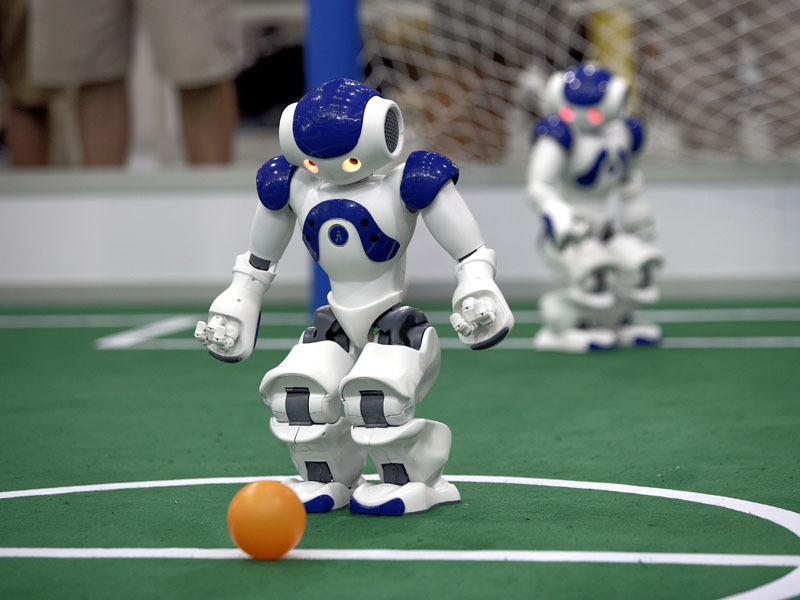
\includegraphics[width=.40\linewidth,height=.30\linewidth]{images/img_10612}}~~~
    \subfigure{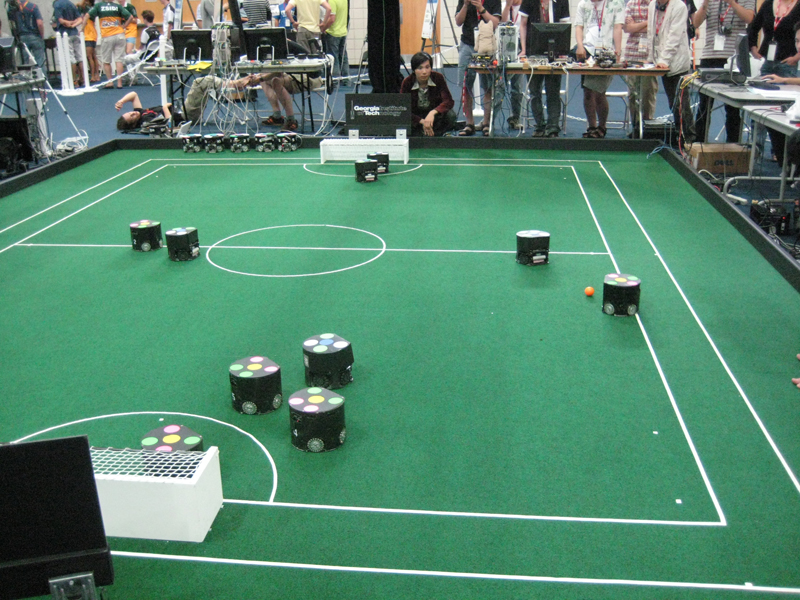
\includegraphics[width=.40\linewidth,height=.30\linewidth]{images/img_08482}}
    ~\\
    \subfigure{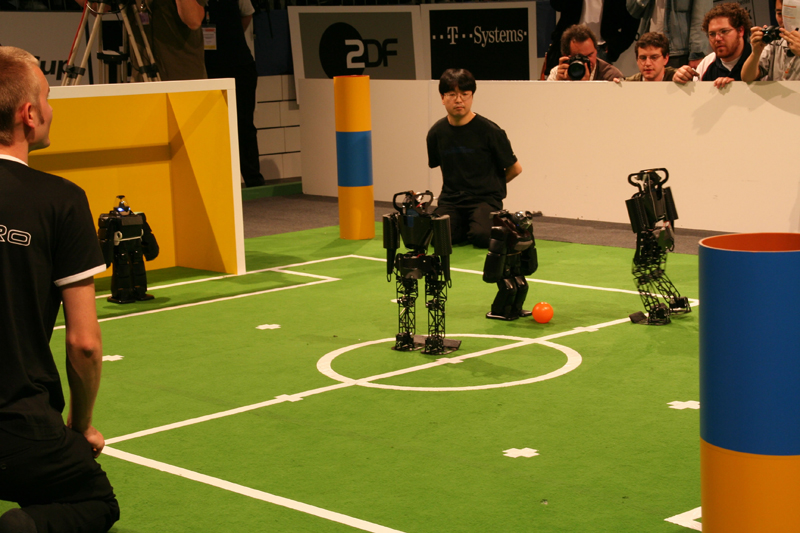
\includegraphics[width=.40\linewidth,height=.30\linewidth]{images/img_6321_jpg}}~~~
    \subfigure{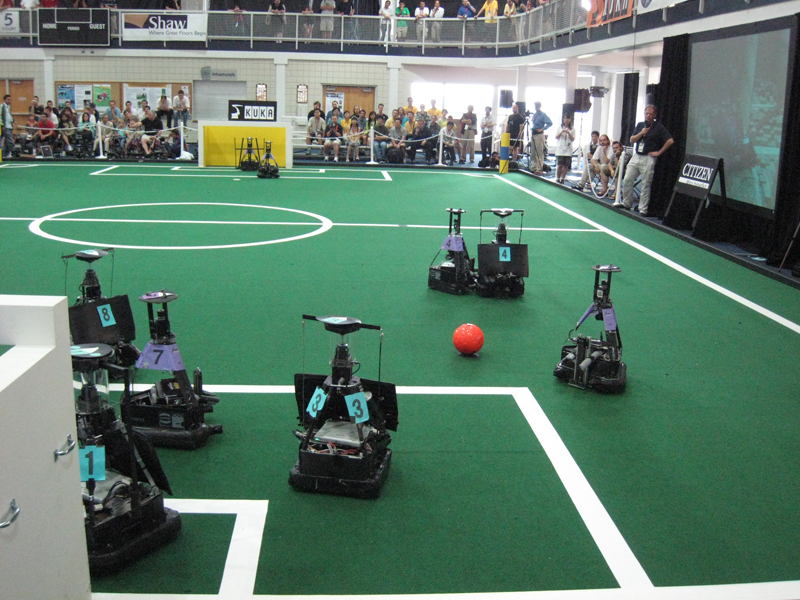
\includegraphics[width=.40\linewidth,height=.30\linewidth]{images/img_14322}}
\end{figure}
\end{frame}


\begin{frame}
\frametitle{Introduction}
\begin{figure}
    \centering
    \subfigure{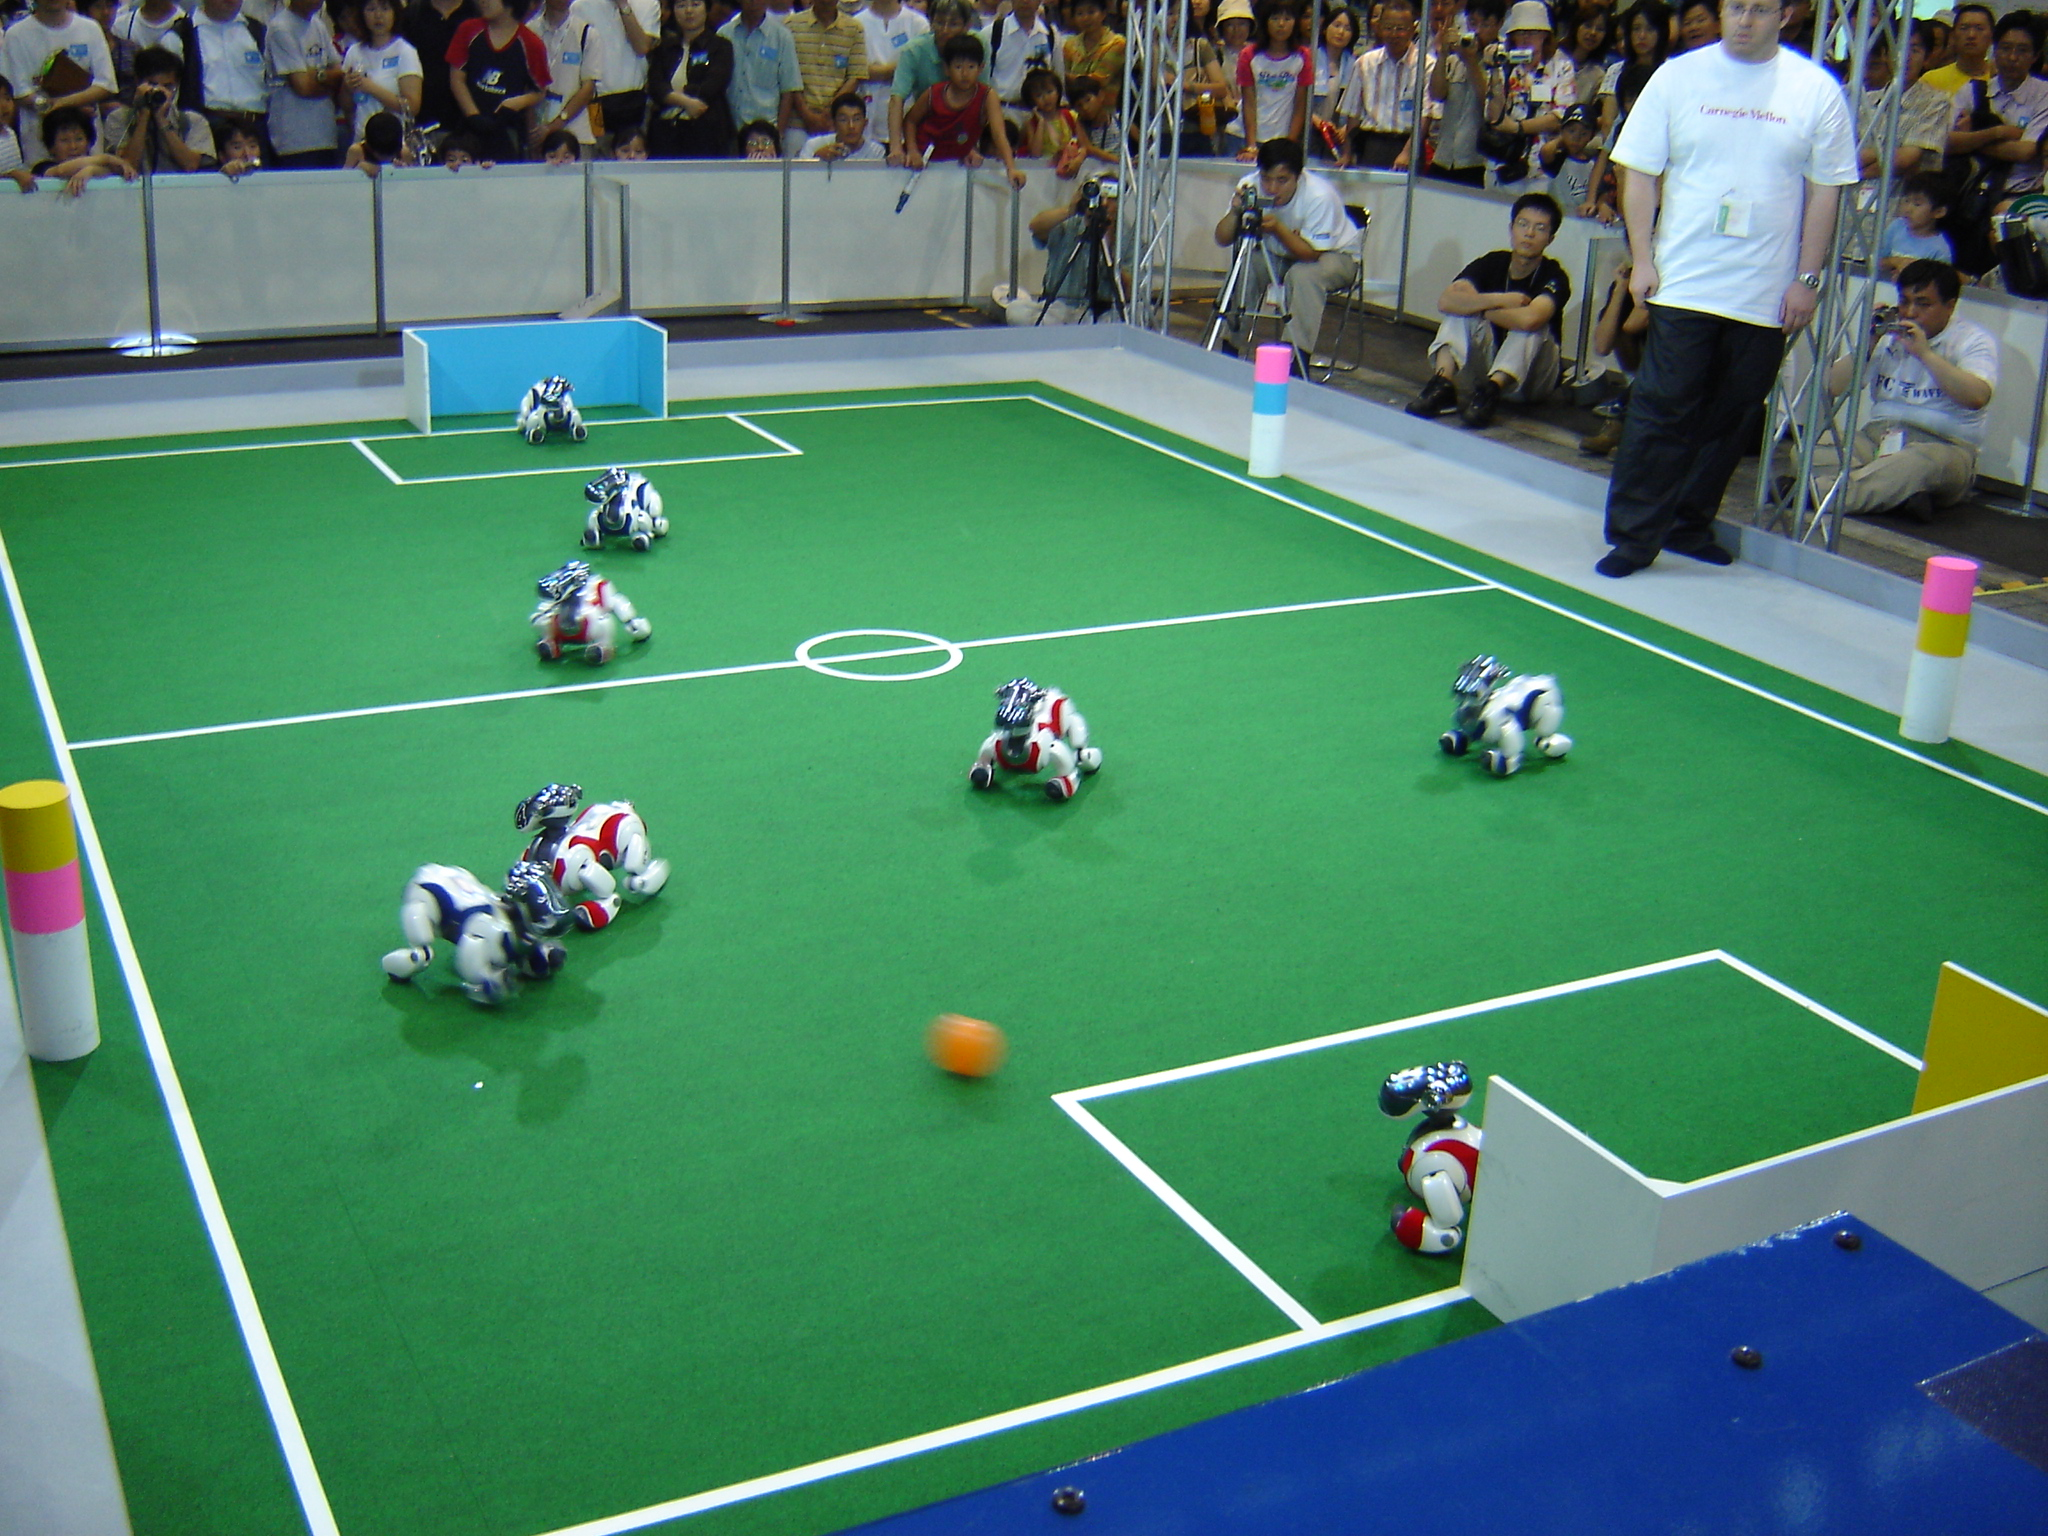
\includegraphics[width=.40\linewidth,height=.30\linewidth]{images/Aibos_playing_football_at_Robocup_2005}}~~~
    \subfigure{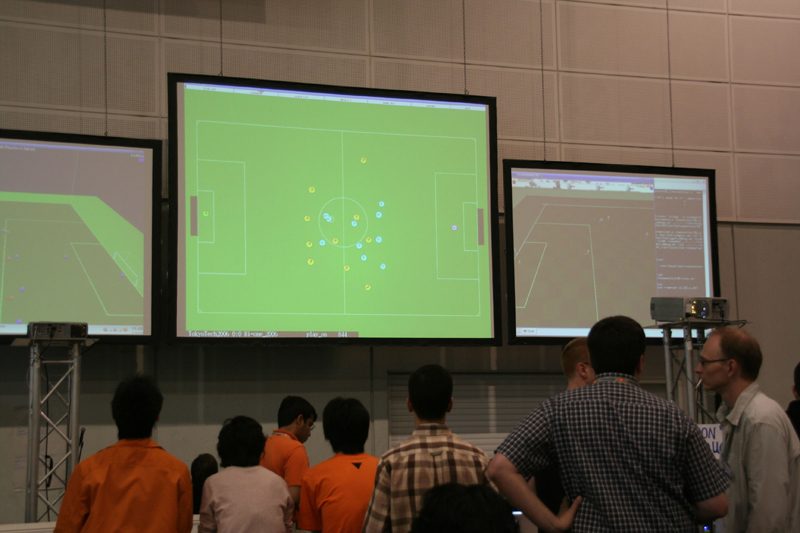
\includegraphics[width=.40\linewidth,height=.30\linewidth]{images/img_5461_jpg}}
    ~\\
    \subfigure{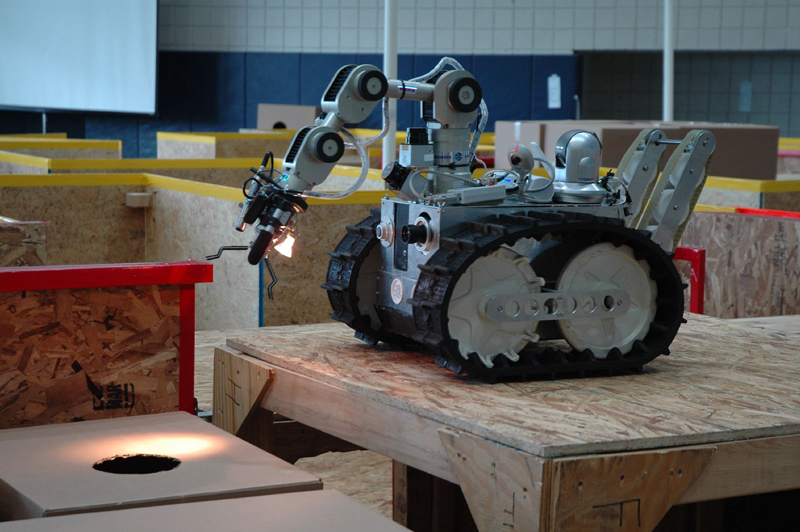
\includegraphics[width=.40\linewidth,height=.30\linewidth]{images/deu_jacobs_asj_08_}}~~~
    \subfigure{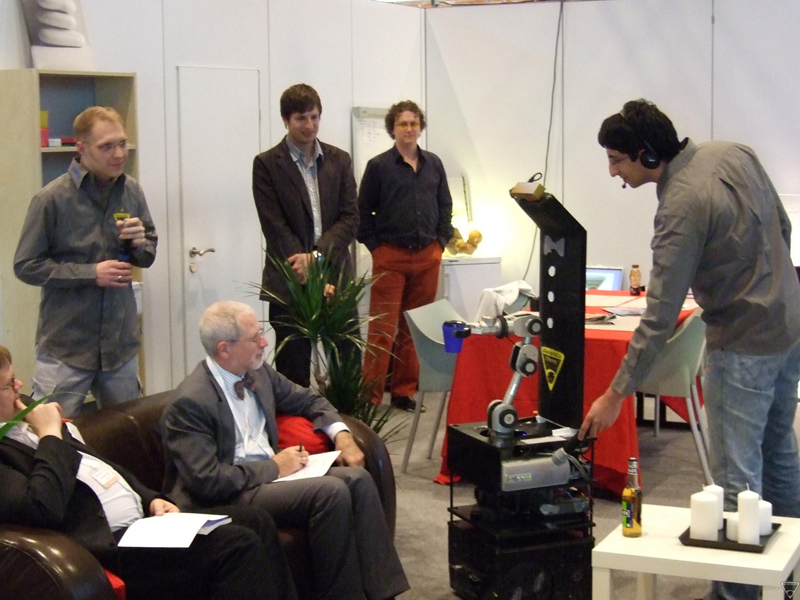
\includegraphics[width=.40\linewidth,height=.30\linewidth]{images/dscf3202}}
\end{figure}
\end{frame}

%%%%%%%%%%%%%%%%%%%%%%%%%%%%%%%%%%%%%%%

\section{Positionnement du problème}
\begin{frame}
\begin{center}
{\LARGE Positionnement du problème}
\end{center}
\end{frame}


\begin{frame}
\frametitle{Le domaine étudié}
Plusieurs agents (robots) qui appartiennent à une même équipe
\begin{itemize}
	\item ils ont des objectifs communs (marquer des buts dans le camp adverse et empêcher les adversaires de marquer)
	\item et des objectifs individuels (défendre une zone, attaquer, etc.)
\end{itemize}
~\\
Coordination (orienté tâche)
\begin{itemize}
	\item permet d'éviter les conflits entre buts individuels et buts collectifs
	\item coopération, interactions positives (synergies) % TODO
	%\item orienté tâche (buts communs, ensemble de rôles)
	%\item distribution dynamique des rôles (réorganisation possible)
\end{itemize}
\end{frame}


%\begin{frame}
%\frametitle{Le domaine étudié}
%Architecture des agents
%\begin{itemize}
%	\item réactif
%	\item délibératif (cognitif)
%	\item hybride
%	\item en couches
%\end{itemize}
%Architecture réactive ou délibérative ?
%\begin{itemize}
%	\item réactive : robots rapides aux comportements simple
%	\item délibérative : modèle globale du monde, résonne, coordination
%\end{itemize}
%\end{frame}


\begin{frame}
\frametitle{La coordination des agents}
\begin{columns}
    \begin{column}{0.3\textwidth}
        \begin{center}
                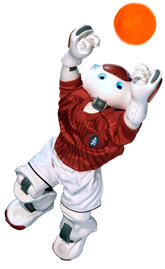
\includegraphics[width=.90\linewidth]{images/nao3}
        \end{center}
    \end{column}
    \begin{column}{0.6\textwidth}
        Les différents aspects de la coordination
        \begin{itemize}
            \item position
            \item tactique (team formation)
            \begin{itemize}
                \item rôle
                \item comportement (behaviour)
            \end{itemize}
            \item plan
            \begin{itemize}
                \item action
            \end{itemize}
        \end{itemize}
    \end{column}
\end{columns}
\end{frame}


\begin{frame}
\frametitle{La coordination des agents}
Les contraintes
\begin{itemize}
	\item temps réel
	\item environnement très dynamique et imprévisible
	\item communication bruitée
	\item latences importantes dans les communications
	\item bande passante limitée du canal de communication
\end{itemize}
~\\
Les conséquences
\begin{itemize}
	\item décision décentralisée
	\item échanges limités
	\item pas de négociation complexe
	\item autonomie (coupure des communications)
\end{itemize}
\end{frame}


\begin{frame}
\frametitle{Les différentes approches}
\begin{columns}
    \begin{column}{0.75\textwidth}
        \begin{itemize}
            \item behaviour based coordination $[$CAN01$]$
            \begin{itemize}
                \item Qlearning $[$PAR01$]$
                %\item graphs de coordination $[$KOK02$][$KOK03$]$
                %\item strategie collision avoidance $[$SPR97$]$
                \item ANN decision making $[$JOL07$][$ATK09$]$
                \item algorithmes évolutionnistes $[$SON01$]$
                \item fuzzy condition and motivation $[$BON03$][$HUA02$]$
            \end{itemize}
            \item planification distribuée
            \item coordination sans négociation $[$LAU10$]$
        \end{itemize}
    \end{column}
    \begin{column}{0.25\textwidth}
        \begin{center}
                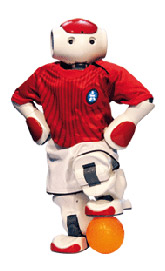
\includegraphics[width=.95\linewidth]{images/nao1}
        \end{center}
    \end{column}
\end{columns}
\end{frame}

%%%%%%%%%%%%%%%%%%%%%%%%%%%%%%%%%%%%%%%

\section{Un exemple de protocole de coordination}
\begin{frame}
\begin{center}
{\LARGE Un exemple de protocole de coordination}
\end{center}
\end{frame}


\begin{frame}
\frametitle{Azzurra Robot Team (ART Team)}
Robocup middle league
\begin{figure}
    \centering
    \subfigure{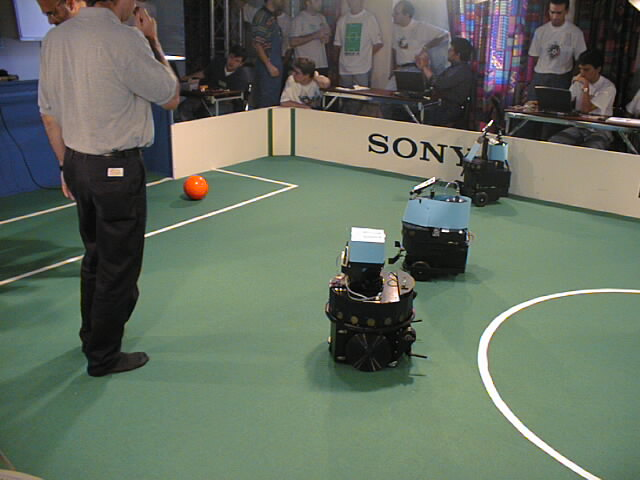
\includegraphics[width=.25\linewidth,height=.20\linewidth]{images/art1}}~~~
    \subfigure{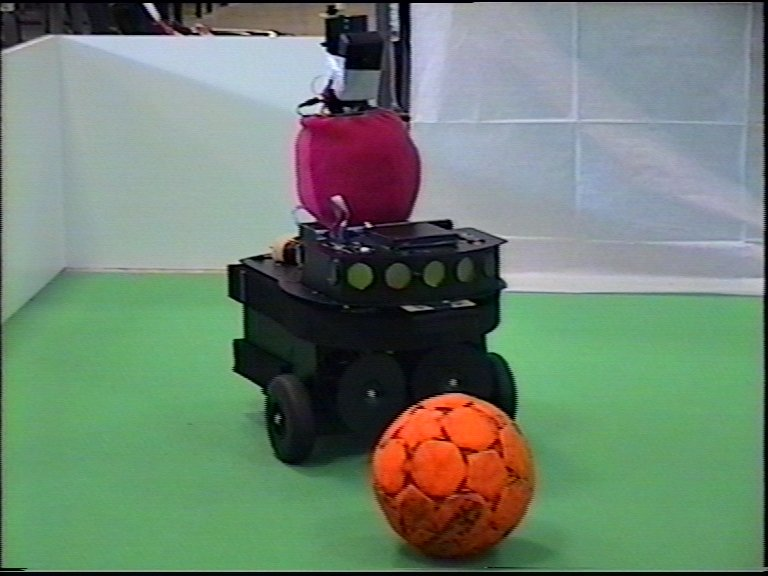
\includegraphics[width=.25\linewidth,height=.20\linewidth]{images/ronaltino}}~~~
    \subfigure{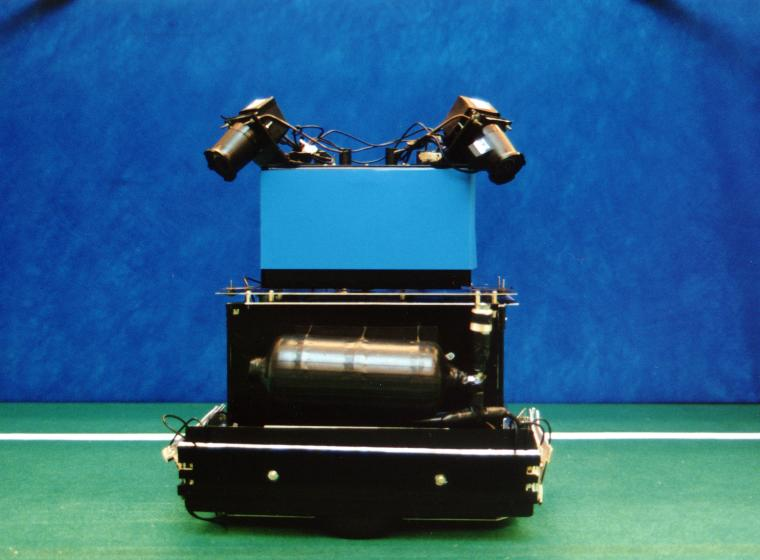
\includegraphics[width=.25\linewidth,height=.20\linewidth]{images/tinozoff}}
\end{figure}
~\\
Particularités
\begin{itemize}
	\item une équipe de robots hétérogène (matériel et logiciel)
	\item robots construits dans 7 universités différentes
\end{itemize}
\end{frame}


\begin{frame}
\frametitle{Objectifs et choix de conception}
Objectifs
\begin{itemize}
	\item robots hétérogènes
    \item décisions distribuées
    \begin{itemize}
         \item autonomie
         \item robustesse
         \item tolérance face aux erreurs communication
    \end{itemize}
    \item répartition des rôles efficace (seulement 1 joueur sur la balle) 
	\item n'importe quel robot peut être remplacé à tout moment sans affecter les performances de l'équipe
\end{itemize}
\end{frame}


\begin{frame}
\frametitle{Objectifs et choix de conception}
Architecture à deux couches (asynchrones)
\begin{itemize}
	\item une couche réactive
	\item une couche délibérative
\end{itemize}
\begin{center}
    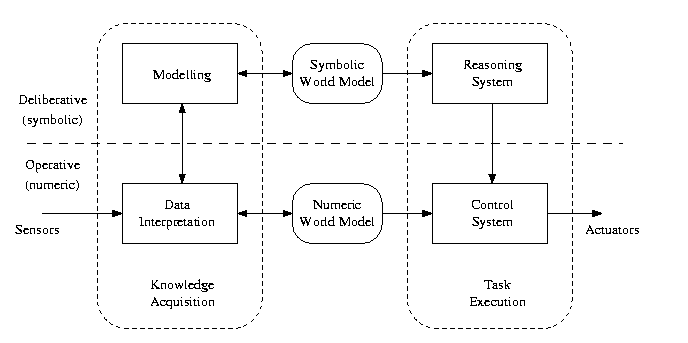
\includegraphics[width=.90\linewidth]{images/art}
\end{center}
\end{frame}


\begin{frame}
\frametitle{Objectifs et choix de conception}
\begin{center}
    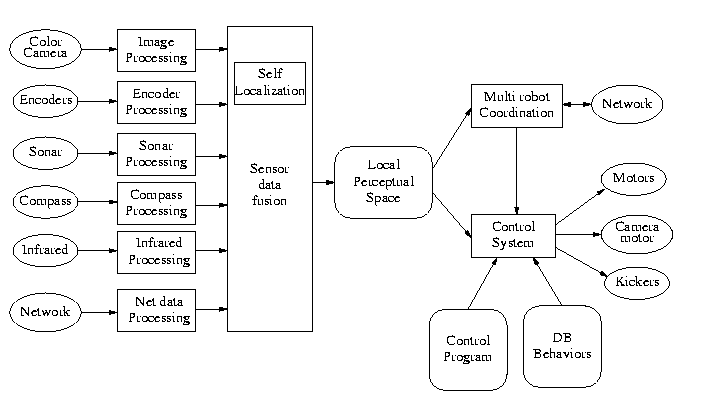
\includegraphics[width=.90\linewidth]{images/art_sw}
\end{center}
\end{frame}


\begin{frame}
\frametitle{Rôles, formations et stratégie}
Rôles
\begin{itemize}
	\item défenseur
    \item milieu de terrain
    \item attaquant
\end{itemize}
~\\
Formations
\begin{itemize}
	\item détermine les rôles à distribuer (exemple : 1-2-1)
    \item chaque robot peut jouer n'importe quel rôle
    \item le rôle des robots change au cours de la partie
\end{itemize}
~\\
Stratégies
\begin{itemize}
	\item offensive
    \item défensive
\end{itemize}
\end{frame}


\begin{frame}
\frametitle{Stratégies et rôles}
Contraintes
\begin{itemize}
	\item le protocole de coordination est distribué
	\item deux robots ne doivent pas prendre le même rôle (conflits)
	\item tous les rôles doivent être distribués
	\item les rôles sont attribués dynamiquement, par communication explicite
	%\item échanges de messages
    \item négociation simplifiée
\end{itemize}

Deux étapes $[$CAN01$]$
\begin{itemize}
	\item choix de la formation
	\item affectation des rôles
\end{itemize}
\end{frame}


\begin{frame}
\frametitle{Choix de la formation}
Les robots ont un ensemble de règles permettant de choisir une formation
%suivant la configuration de la partie
\begin{itemize}
	\item chaque robot vote pour la meilleure formation
	\item le vote est communiqué par broadcast (pas de négociation)
	\item la formation qui reçoit le plus de vote est choisie
\end{itemize}
\end{frame}


\begin{frame}
\frametitle{Affectation des rôles}
\begin{itemize}
	\item n robots $\{R_1, \dots, R_n\}$
	\item m rôles $\{r_1, \dots, r_m\}$ classés par ordre d'importance pour la formation courante
	\item $f_j(i)$ : fonction d'utilité calculée par le robot $R_i$ pour le rôle $r_j$
	\item $A(i) = j$ : $r_j$ est assigné à $R_i$
\end{itemize}
\begin{center}
    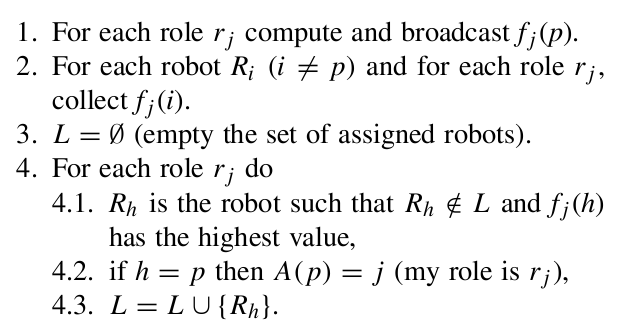
\includegraphics[width=.70\linewidth]{images/algo}
\end{center}
\end{frame}


\begin{frame}
\frametitle{Assignation des rôles}
Stabilité des assignations
\begin{itemize}
    \item l'utilité des rôles est calculée en fonction des perceptions
    \item ces paramètres numériques sont bruités et peuvent osciller
    \item perte de communication
    \item les rôles changent trop souvent
\end{itemize}
Augmenter le poids du rôle courant dans la fonction d'utilité de chaque robot (hysteresie)\\
~\\
Incapacité à exécuter un rôle
\begin{itemize}
    \item robot bloqué par un autre joueur, \dots
\end{itemize}
Céder le rôle courant en diminuant son poids dans la fonction d'utilité
\end{frame}


\begin{frame}
\frametitle{Résultats}
Enregistrement d'un match de la robocup européenne (2000)
\begin{center}
    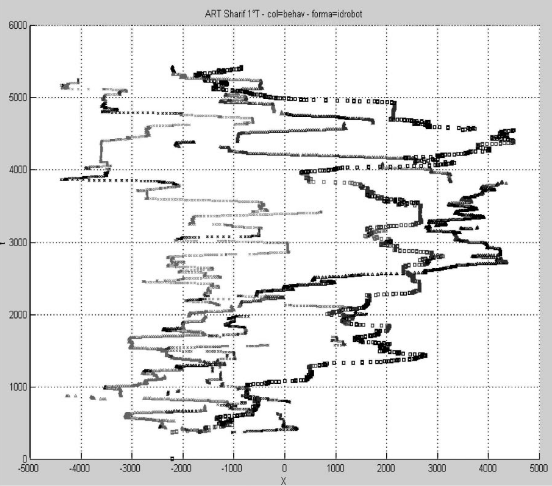
\includegraphics[width=.70\linewidth]{images/log}
\end{center}
\end{frame}


\begin{frame}
\frametitle{Résultats}
Les objectifs sont atteints
\begin{itemize}
    \item les rôles sont rarement vaquants
    \item les robots se retrouvent rarement sans rôle
    \item les changements de rôles sont fluides
\end{itemize}
~\\
Limites et critiques
\begin{itemize}
    \item la fiabilité du groupe dépend trop de la fiabilité des agents
    %erreurs de perceptions entraînent une mauvaise attribution des rôles
    %\item indice de fiabilité (robot hétérogène)
    \item pas d'apprentissage $[$JOL07$]$
    \item trop de communication explicite $[$LAU10$]$
    \item ne tient pas compte de l'équipe adverse $[$ATK09$]$
\end{itemize}
\end{frame}

%%%%%%%%%%%%%%%%%%%%%%%%%%%%%%%%%%%%%%%

\begin{frame}
\frametitle{Conclusion}
La robocup est un cadre intéressant pour tester les protocoles de coordination.\\
~\\
Elle impose des contraintes fortes et proches de ce qu'on attend dans de nombreuses applications\\
~\\
Les protocoles utilisés sont efficaces mais la marge de progression reste importante.
\end{frame}


\begin{frame}[allowframebreaks]
\frametitle{Bibliographie}
\begin{itemize}
    \item $[$KIT98$]$
    Kitano, H. and Tambe, M. and Stone, P. and Veloso, M. and Coradeschi, S. and Osawa, E. and Matsubara, H. and Noda, I. and Asada, M.,
    \emph{{The RoboCup synthetic agent challenge 97}}, Lecture Notes in Computer Science \textbf{1395} (1998), Springer, p.62--73.

	\item $[$BON03$]$
	T.~Halva~Labella A.~Bonarini, G.~Invernizzi and M.~Matteucci.
	 An architecture to coordinate fuzzy behaviors to control an
	  autonomous robot.
	 \em Fuzzy sets and systems, 134(1):101--115, 2003.

	\item $[$ATK09$]$
	J.~Atkinson and D.~Rojas.
	 On-the-fly generation of multi-robot team formation strategies based
	  on game conditions.
	 \em Expert Systems with Applications, 36(3P2):6082--6090, 2009.

	\item $[$CAN01$]$
	L.~Iocchi D.~Nardi C.~Candea, H.~Hu and M.~Piaggio.
	 Coordination in multi-agent RoboCup teams.
	 \em Robotics and Autonomous Systems, 36(2-3):67--86, 2001.

	\item $[$KIT98$]$
	P.~Stone M. Veloso S. Coradeschi E. Osawa H. Matsubara I.~Noda H.~Kitano,
	  M.~Tambe and M.~Asada.
	 The RoboCup synthetic agent challenge 97.
	 \em Lecture Notes in Computer Science, 1395:62--73, 1998.

	\item $[$HUA02$]$
	H.P. Huang and C.C. Liang.
	 Strategy-based decision making of a soccer robot system using a
	  real-time self-organizing fuzzy decision tree.
	 \em Fuzzy Sets and Systems, 127(1):49--64, 2002.

	\item $[$JEO97$]$
	I.K. Jeong and J.J. Lee.
	 Evolving cooperative mobile robots using a modified genetic
	  algorithm.
	 \em Robotics and autonomous systems, 21(2):197--205, 1997.

	\item $[$JOL07$]$
	KG~Jolly, KP~Ravindran, R.~Vijayakumar, and R.~Sreerama~Kumar.
	 Intelligent decision making in multi-agent robot soccer system
	  through compounded artificial neural networks.
	 \em Robotics and Autonomous Systems, 55(7):589--596, 2007.

	\item $[$KOK02$]$
	M.T.J~Spaan J.R.~Kok and N.~Vlassis.
	 An approach to noncommunicative multiagent coordination in
	  continuous domains.
	 In \em Benelearn, pages 46--52. Citeseer, 2002.

	\item $[$KOK03$]$
	M.T.J~Spaan J.R.~Kok and N.~Vlassis.
	 Multi-robot decision making using coordination graphs.
	 In \em Proceedings of the 11th International Conference on Advanced
	  Robotics, ICAR, volume~3, pages 1124--1129. Citeseer, 2003.

	\item $[$PAR01$]$
	Y.J.~Kim K.H.~Park and J.H. Kim.
	 Modular Q-learning based multi-agent cooperation for robot soccer.
	 \em Robotics and Autonomous Systems, 35(2):109--122, 2001.

	\item $[$LAU10$]$
	M.~Lauer, R.~Hafner, S.~Lange, and M.~Riedmiller.
	 Cognitive Concepts in Autonomous Soccer Playing Robots.
	 \em Cognitive Systems Research, 2010.

	\item $[$SON01$]$
	K.T. Song and C.C. Tang.
	 Learning for cooperation in multirobot team competitions.
	 In \em Computational Intelligence in Robotics and Automation, 2001.
	  Proceedings 2001 IEEE International Symposium on, pages 302--307, 2001.

	\item $[$SPR97$]$
	G.~Springer, P.~Hannah, RJ~Stonier, S.~Smith, and P.~Wolfs.
	 Simple strategies for collision-avoidance in robot soccer.
	 \em Robotics and autonomous systems, 21(2):191--196, 1997.
\end{itemize}
\end{frame}

%\begin{frame}
%%\frametitle{Licences}
%\begin{center}
%    \href{http://creativecommons.org/licenses/by-sa/2.0/fr/}{
\includegraphics[width=.40\linewidth]{images/cc_by_sa}}
%    \\[3em]
%%    \textbf{Illustrations}\\\medskip
%%    \href{http://commons.wikimedia.org/wiki/User:Nojhan}{Johann "nojhan" Dréo} \raisebox{-0.5\height+0.3em}{\href{http://creativecommons.org/licenses/by-sa/2.0/fr/}{
\includegraphics[height=1em]{images/cc_by_sa_small}}}
%\end{center}
%\end{frame}

\end{document}
